\section{Decision-tree methods}
This methods don't rely on any assumption on the data, they just try to split the space to obtain the best classification/regression possible. To do that it splits the predictor space in regions $R_1,R_2...R_M$ and the prediction for each region is the mean of the datapoints in it.
$$
\hat{y}_{R_m} = \frac{1}{|R_m|} \sum_{i: x_i \in R_m} y_i
$$
\begin{figure}[h]
    \centering
    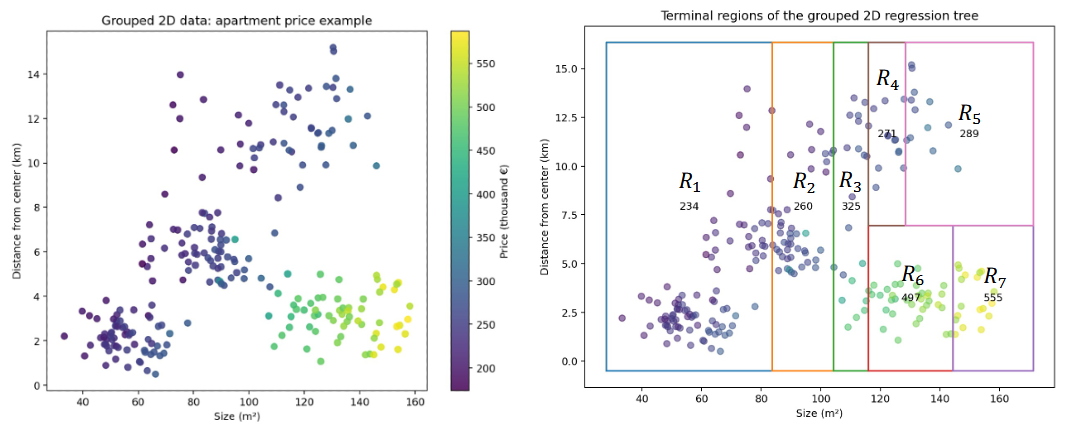
\includegraphics[width=0.75\linewidth]{img//tree-models//decision-tree/decision_tree.png}
\end{figure}
\begin{figure}[h]
    \centering
    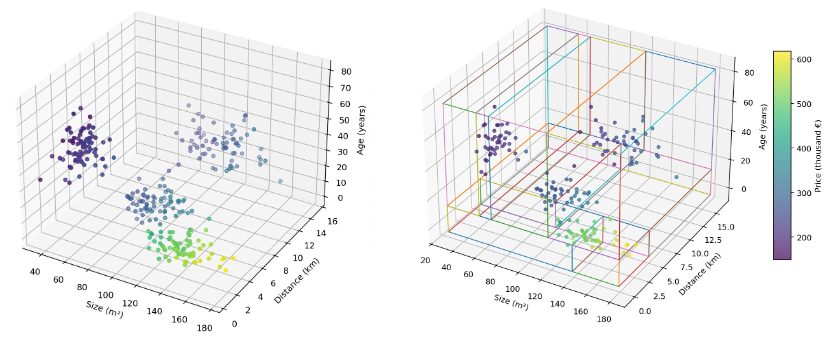
\includegraphics[width=0.75\linewidth]{img//tree-models//decision-tree/decision_tree_3d.png}
\end{figure}
The splits are \textit{axis-align}: all the splits are the type of $R_s\le s$, allwoing us to dividing the space only hyperplanes. However the non-linearity and complex splits arise from the interaction of \diff splits\textcolor{gray}{(think about the geometry of optimization problems in FOR)}.\\
\newpage
It's called a \textbf{piecewise-constant model} 'cause the predition is a sort of step function with a finite set of values as prediction.
\begin{figure}[h]
    \centering
    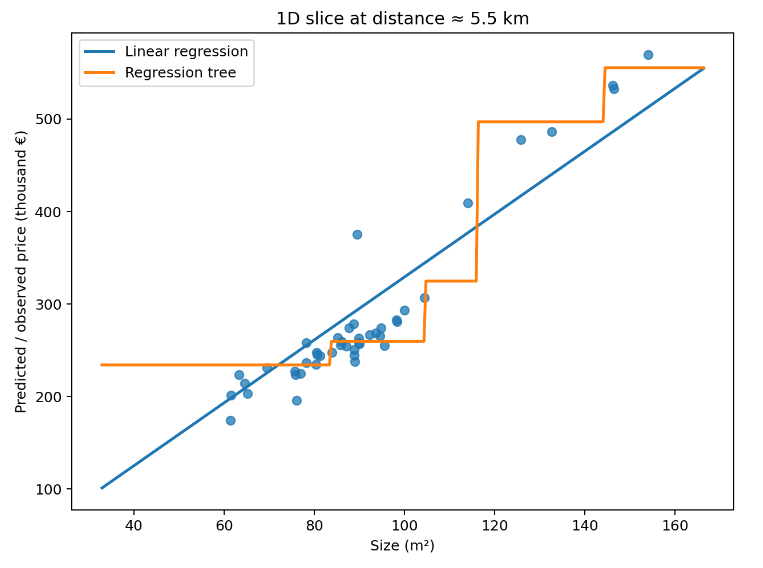
\includegraphics[width=0.3\linewidth]{img//tree-models//decision-tree/dectree_prediction_line.png}
\end{figure}

The same function can be described equivalently using binary trees:
\begin{figure}[h]
    \centering
    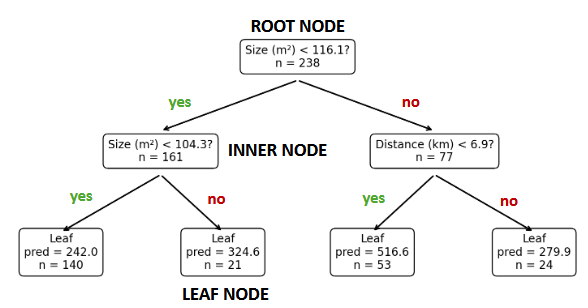
\includegraphics[width=0.4\linewidth]{img//tree-models//decision-tree/decision_tree_mathmodel.png}
\end{figure}\hfill\\
For what concerns \textbf{classification} each leaf node predicts $\hat{y}=\text{majority class}$ and we can estimate $\mathbb{P}(Y=\hat{y}|X\in R_m)=\# \text{ class }\hat{y}\ / \#\text{ total observations }$.


\subsection{Regression tree-fit: binary splitting}
As usual the goal is to minimize the RSS error:
$$
\text{RSS} = \sum_{j=1}^{J} \sum_{i \in R_j} (y_i - \hat{y}_{R_j})^2
$$
however doing so requires to try out all the possible combos of splitting, which is unfeasible \arrow we have to approach the problem using a top-down, greedy algorithm known as \textbf{recursive binary splitting}.
\vspace{0.2cm}
At each step we choose a predictor, we take all the possible thresholds and we select the one that gives us the largest reduction in prediction error:
$$
(j^*, s^*) = \arg\min_{j,s} \text{RSS}(j,s) = \arg\min_{j,s}\sum_{x_{x_i} \in R_L(j,s)} (y_i - \bar{y}_{R_L})^2 + \sum_{x_{x_i} \in R_R(j,s)} (y_i - \bar{y}_{R_R})^2
$$
\begin{figure}[h]
    \centering
    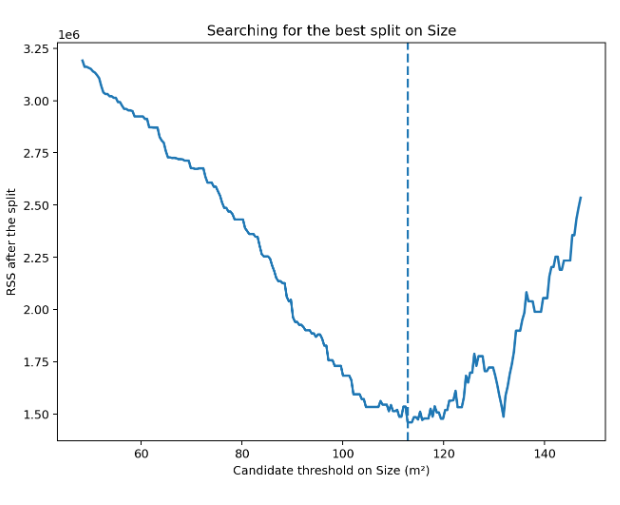
\includegraphics[width=0.35\linewidth]{img//tree-models//decision-tree/dectree_threshold_selection.png}
\end{figure}
\newpage
Technically we can continue forever with the splitting, but when do we stop? There are several criterions:
\begin{itemize}
    \item min num of obs required to split: $|R_m|<n_{min}^{split}$ 
    \item min num of obs allowed in each terminal node \textcolor{gray}{(dont't do the split if I end up with something too small)}: $|R_L|<n_{min}^{leaf},\ \  |R_R|<n_{min}^{leaf}$
    \item max tree depth: $depth(R_m)\ge d_{max}$
    \item min improvement: $\max_{j,s} \Delta \text{RSS}(j,s) = \max_{j,s} \text{RSS}(R_m) - [\text{RSS}(R_L(j,s)) + \text{RSS}(R_R(j,s))] < \varepsilon$ 
\end{itemize}

\subsection{Decision-tree complexity control}
As in all the models, we have to controll the complexity 'cause as the number of leaf increases the validation error might increase. The idea is to build the tree as far as our stopping criterion allows us, and then we trim some leafs.

\subsubsection{Cost-complexity pruning}
The goal is to minimize not only the erro but also the number of leafs ($\alpha$ is an hyperparam and it's selected using cross-validation):\\
$$
\text{RSS}(T)+\alpha |T|\quad |T| := \text{num terminal nodes}
$$
\vspace{0.2cm}
Then we start from a large tree $T_0$ we generate a sequence of sub-trees $T_0 \supset T_1 \supset T_2 \supset \cdots \supset T_L$ as follows: for each internal node $t$ consider the sub-tree rooted in it $T_t$, then compute the RSS by keeping that subtree and the RSS by removing it, and compute the following, choosing the lowest one.
$$
g(t) = \frac{RSS(t)-RSS(T_t)}{|\bar{T_t}|-1} := \text{pruning cost per leaf removed}
$$
\begin{figure}[h]
    \centering
    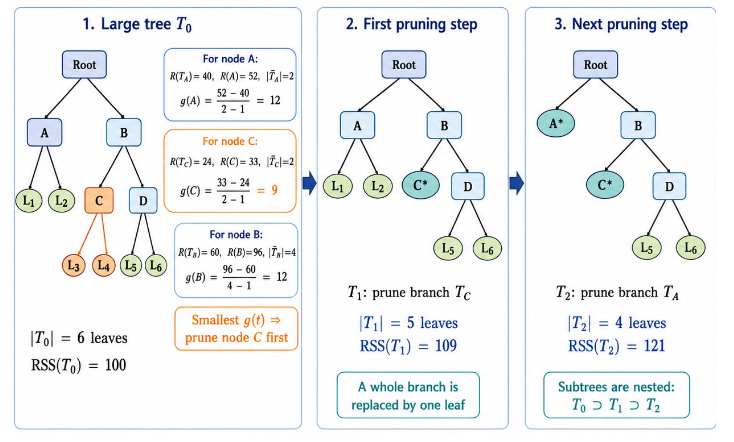
\includegraphics[width=0.75\linewidth]{img//tree-models//decision-tree/cost_complexity_pruning.png}
\end{figure}

\newpage
Each of the trees obtained is optimal for some range of $\alpha$ for the cost-complexity metric:
\begin{figure}[h]
    \centering
    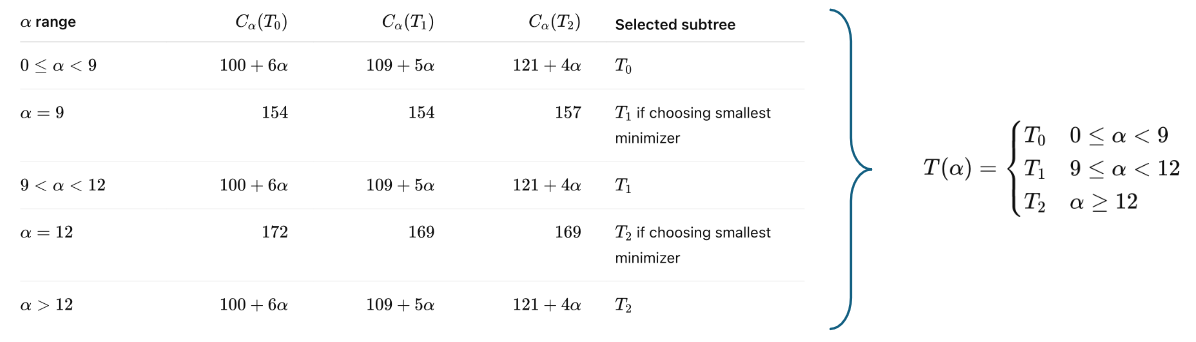
\includegraphics[width=0.75\linewidth]{img//tree-models//decision-tree/alpha_selection.png}
\end{figure}\hfill\\
and in the end we select using cross-validation $\hat{\alpha}=\arg\min_{\alpha}CV(\alpha)$, choosing the subtree among the candidate pruned subtrees for that $\alpha$ value.

\vspace{0.3cm}
\subsubsection{Feature selection using decision trees}
Trees can be used also for selecting relevant features: during the branch construction only some variables are used, so if a predictor never appears in a split it means it doesn't contribute to the prediction. However the variable selection might be unstable, so we have to select the predictors based on some average execution.
\begin{figure}[h]
    \centering
    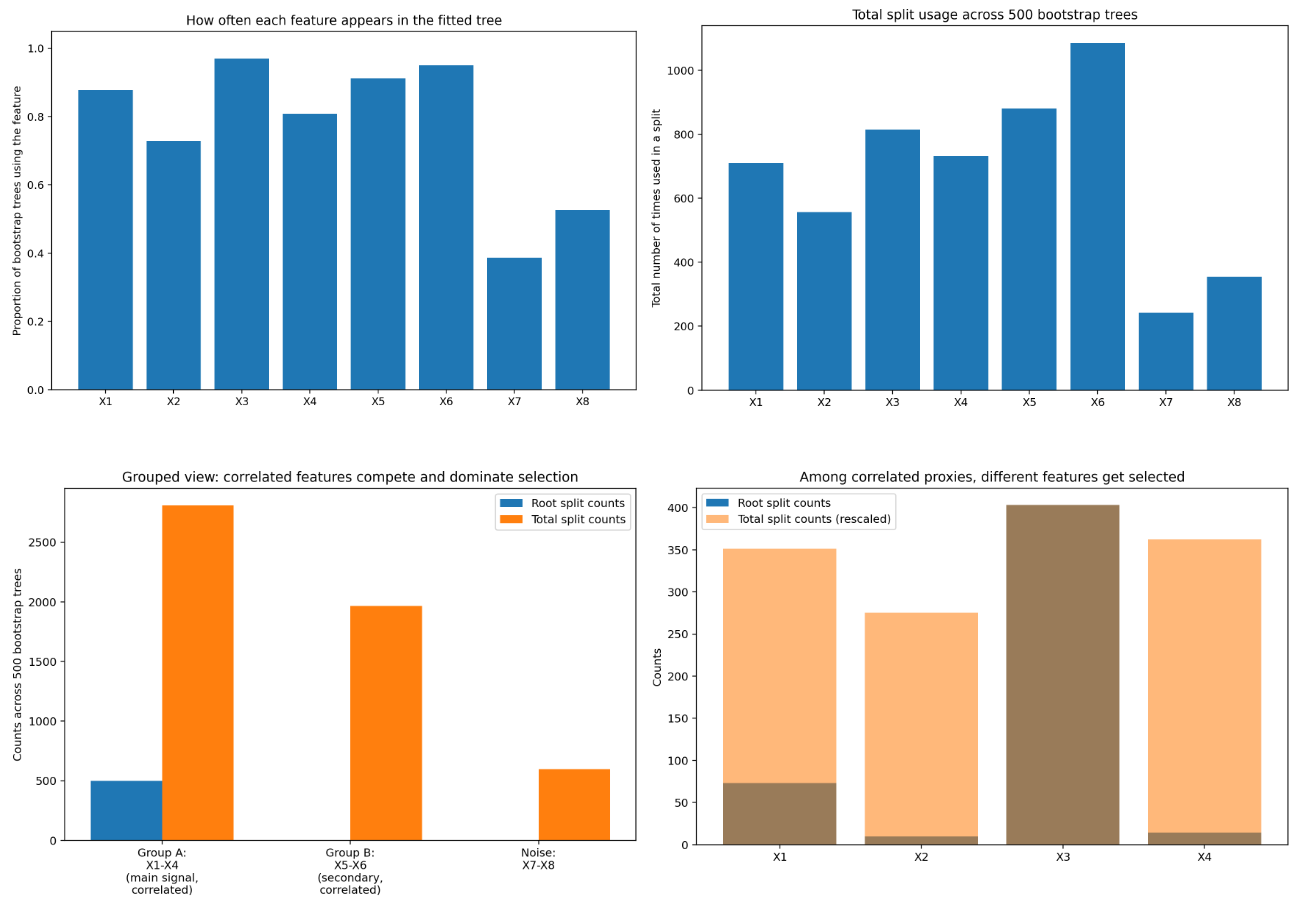
\includegraphics[width=0.85\linewidth]{img//tree-models//decision-tree/dectree_feature_selection.png}
\end{figure}

\subsubsection{Pro \& Cons: decision trees}
\begin{minipage}[t]{0.45\textwidth}
\textcolor{green}{\textbf{Pro:}}
\begin{itemize}
    \item are easy to explain
    \item produce if-then rules
    \item handle nonlinear effects
    \item capture interactions automatically
    \item do not require feature scaling \textcolor{gray}{(they handle one predictor at a time)}
    \item can handle numerical and categorical predictors
    \item can handle missing values \textcolor{gray}{(prediction are arranged base on the avrage)}
    \item perform a form of embedded feature selection
\end{itemize}
\end{minipage}
\begin{minipage}[t]{0.45\textwidth}
\textcolor{red}{\textbf{Cons:}}
\begin{itemize}
    \item can overfit
    \item are high-variance
    \item may be unstable
    \item produce stepwise predictions
    \item can be sensitive to small changes in the training data
\end{itemize}
\end{minipage}